\documentclass[../TDT5.tex]{subfiles}%

\begin{document}
\section{Moteur à explosion -- cycle de Beau de \textsc{Rochas}}
\enonce{%
	Dans un moteur à explosion, $n$ moles de gaz parfait subit le cycle de
	\textsc{Beau de Rochas}, composé de deux adiabatiques et de deux isochores~:
	\begin{itemize}
		\item compression adiabatique de l'état $(P_1,V_1,T_1)$ à l'état
		      $(P_2,V_2,T_2)$~;
		\item échauffement isochore de l'état $(P_2,V_2,T_2)$ à l'état
		      $(P_3,V_3,T_3)$~;
		\item détente adiabatique de l'état $(P_3,V_3,T_3)$ à l'état $(P_4,V_4,T_4)$~;
		\item refroidissement isochore qui ramène le fluide à l'état initial.
	\end{itemize}
	Les transformations sont supposées quasi-statiques.
}%
\QR{%
	Représenter le cycle dans un diagramme de \textsc{Watt} $(P,V)$.
}{%
	\sswitch{
		\hfill
		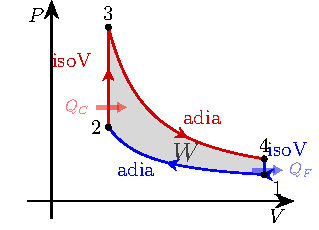
\includegraphics[width=.5\linewidth, valign=t]{E3_PV_bdr}
		\hspace*{\fill}
	}{
		\vspace{-15pt}
		\begin{center}
			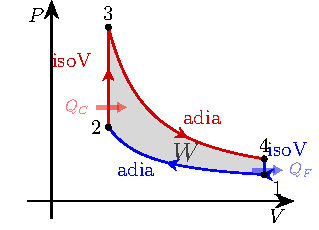
\includegraphics[width=.5\linewidth, valign=t]{E3_PV_bdr}
		\end{center}
	}
}%

\QR{%
	Exprimer les travaux et transferts thermiques au cours des différentes
	étapes en fonction $n,R,\gamma$ et des températures. En déduire le
	rendement théorique $r$ de ce cycle en fonction des températures
	$T_1$, $T_2$, $T_3$ et $T_4$.
}{%
	Pour les adiabatiques, $Q = 0$, et pour les isochores, $W = 0$. De plus,
	$\Delta{U} = C_V\Delta{T}$ et $C_V = \frac{nR}{\gamma-1}$.
	\vspace{10pt}
	\begin{itemize}
		\item $1\to 2$~:
		      \leavevmode\vspace*{-20pt}\relax
		      \[
			      Q_{12} = 0
			      \Ra
			      \boxed{W_{12} = \Delta{U}_{12} = \frac{nR}{\gamma-1}(T_2-T_1)}
		      \]
		      \vspace{10pt}
		\item $2\to 3$~:
		      \leavevmode\vspace*{-20pt}\relax
		      \[
			      W_{23} = 0
			      \Ra
			      \boxed{Q_{23} = \Delta{U}_{23} = \frac{nR}{\gamma-1}(T_3-T_2)}
		      \]
		      \vspace{10pt}
		\item $3\to 4$~:
		      \leavevmode\vspace*{-20pt}\relax
		      \[
			      Q_{34} = 0
			      \Ra
			      \boxed{W_{34} = \frac{nR}{\gamma-1}(T_4-T_3)}
		      \]
		      \vspace{10pt}
		\item $4\to 1$~:
		      \leavevmode\vspace*{-20pt}\relax
		      \[
			      W_{41} = 0
			      \Ra
			      \boxed{Q_{41} = \frac{nR}{\gamma-1}(T_1-T_4)}
		      \]
	\end{itemize}
	Pour un moteur,
	\[
		r = -\frac{W\ind{tot}}{Q_C}
		\qet
		Q_C = Q_{23}
	\]
	car $Q_{23} > 0$ et $Q_{41} < 0$. Ainsi,
	\begin{gather*}
		r =
		- \cancel{\frac{nR}{\gamma-1}}(T_2-T_1+T_4-T_3) \times
		\cancel{\frac{\gamma-1}{nR}}\times
		\frac{1}{T_3-T_2}
		\\\Lra
		r = \frac{T_3+T_1-T_2-T_4}{T_3-T_2}
		\\\Lra
		\boxed{r = 1+\frac{T_1-T_4}{T_3-T_2}}
	\end{gather*}
}%

\QR{%
	En déduire l'expression de $r$ en fonction du rapport volumétrique $x =
		\frac{V_1}{V_2}$ et du coefficient adiabatique $\gamma =
		\frac{C_P}{C_V}$ du fluide.
}{%
	Sur les adiabatiques quasi-statiques du gaz parfait, on a des transformations
	isentropiques donc on applique la loi de \textsc{Laplace}~: $PV^{\gamma} =
		\cte \Lra TV^{\gamma-1} = \cte$~:
	\smallbreak
	\begin{isd}
		\begin{DispWithArrows*}
			T_3V_3^{\gamma-1} &= T_4V_4^{\gamma-1}
			\Arrow{Isochores}
			\\\Lra
			T_3V_2^{\gamma-1} &= T_4V_1^{\gamma-1}
			\\\Lra
			\left( \frac{V_1}{V_2} \right)^{\gamma-1} &= \frac{T_3}{T_4}
			\Arrow{$x = \frac{V_1}{V_2}$}
			\\\Lra
			\Aboxed{T_3 &= T_4 x^{\gamma-1}}
		\end{DispWithArrows*}
		\tcblower
		De même,
		\begin{DispWithArrows*}
			T_1V_1^{\gamma-1} &= T_2V_2^{\gamma-1}
			\\\Lra
			\left( \frac{V_1}{V_2} \right)^{\gamma-1} &= \frac{T_2}{T_1}
			\\\Lra
			\Aboxed{T_2 &= T_1 x^{\gamma-1}}
		\end{DispWithArrows*}
	\end{isd}
	Ainsi,
	\vspace{-20pt}
	\begin{DispWithArrows*}
		r &= 1+\frac{T_1-T_4}{(T_4-T_1)x^{\gamma-1}}
		\\\Lra
		\Aboxed{r &= 1 - x^{1-\gamma}}
	\end{DispWithArrows*}
}%

\begin{blocQR}
	\item \enonce{%
		Le piston du cylindre où évolue l'air ($\gamma = \num{1.4}$) a une course
		$\ell = \SI{10}{cm}$, une section $S = \SI{50}{cm^2}$ et emprisonne un
		volume d'air de \SI{100}{cm^3} en fin de compression. Calculer~:
	}%
	\QR{%
		le rendement théorique du cycle~;
	}}
		\]
	}%

	\QR{%
		le travail fourni au cours d'un cycle, si l'air est admis à une
		pression de \SI{1}{bar} et à \SI{300}{K} et si la température
		maximale est de \SI{900}{K}.
	}{%
		\leavevmode\vspace*{-25pt}\relax
		\begin{gather*}
			W\ind{tot} =
			-rQ_C =
			-r \frac{nR}{\gamma-1}(T_3-T_2)
			\\\beforetext{Or,}
			\left\{
			\begin{array}{ll}
				T_2 & = T_1x^{\gamma-1}
				\\\DS
				nR  & = \frac{P_1V_1}{T_1}
			\end{array}
			\right.
			\qav
			\left\{
			\begin{array}{rcl}
				T_1 & = & \SI{300}{K}
				\\
				P_1 & = & \SI{1}{bar} = \SI{1e5}{Pa}
				\\
				V_1 & = & \SI{500}{cm^3} = \SI{500e-6}{m^3}
			\end{array}
			\right.\\
			\beforetext{Soit}
			\boxed{
				W\ind{tot} =
				-\left( \frac{1-x^{1-\gamma}}{\gamma-1} \right)
				\frac{P_1V_1}{T_1}
				(T_3-T_1x^{\gamma-1})
			}
			\qav
			\left\{
			\begin{array}{rcl}
				x      & = & 5
				\\
				\gamma & = & \num{1.4}
				\\
				T_3    & = & \SI{900}{K}
			\end{array}
			\right.\\
			\AN
			\xul{
				W = -\SI{65.1}{J}
			}
		\end{gather*}
	}%
\end{blocQR}
\end{document}
